% set \papertrue when printing to paper

\newif\ifpaper
% \papertrue
\paperfalse
\ifpaper
\PassOptionsToClass{handout}{beamer}
\fi

%%%%%%%%%%%%%%%%%%%%%%%%%%%%%%%%%%%%%%%%%%%%%%%%%%%%%%%%%%%%%%%%%%%%%%%%%%%%%%%%

\documentclass[hyperref={colorlinks}]{beamer}
\usepackage[T1]{fontenc}
\usepackage{arev}
\usepackage{textcomp}
\usepackage{ragged2e}
\usepackage{tikz}
%\usepackage{hyperref}
\usetikzlibrary{positioning}

%%%%%%%%%%%%%%%%%%%%%%%%%%%%%%%%%%%%%%%%%%%%%%%%%%%%%%%%%%%%%%%%%%%%%%%%%%%%%%%%

\author{Pasquale Claudio Africa\protect\\{\small By: Antonio Cervone and Luca Formaggia}}
\title{A (maybe not so) gentle introduction to git}
\date{22/05/2020}
\pgfdeclareimage[width=0.8\textwidth]{gitdict}{figures/dict.pdf}
\titlegraphic{\pgfuseimage{gitdict}}

%%%%%%%%%%%%%%%%%%%%%%%%%%%%%%%%%%%%%%%%%%%%%%%%%%%%%%%%%%%%%%%%%%%%%%%%%%%%%%%%

\usefonttheme{professionalfonts}
\setbeamertemplate{navigation symbols}{}
\setbeamercolor{shell}{fg=black,bg=black!20}
\setbeamercolor{separation line}{use=structure,bg=structure.fg}

%%%%%%%%%%%%%%%%%%%%%%%%%%%%%%%%%%%%%%%%%%%%%%%%%%%%%%%%%%%%%%%%%%%%%%%%%%%%%%%%

% make _ (underscore) a common character (math does not work here!)
\makeatletter
\catcode`\_=12

\newenvironment{shell}{%
\footnotesize\flushleft\hrule height 0.1ex
\tt\begin{beamercolorbox}[sep=1ex,left]{shell}%
}{%
\end{beamercolorbox}
\hrule height 0.1ex
\endflushleft\par
}

%%%%%%%%%%%%%%%%%%%%%%%%%%%%%%%%%%%%%%%%%%%%%%%%%%%%%%%%%%%%%%%%%%%%%%%%%%%%%%%%

\newcommand*{\tshell}[1]{{\usebeamercolor[fg]{shell}\colorbox{bg}{\tt#1}}}

\newcommand*{\psone}[1][ant]{\$>~}
\newcommand*{\nl}{\textbackslash\\>~}
\newcommand*{\var}[1]{{\it<#1>}}

\newcommand*{\boxltr}[1]{
{\usebeamercolor[fg]{frametitle}
\tikz[remember picture,baseline=(t@mp.base),minimum width=3ex,minimum height=3ex] 
\node [fill=bg,draw=fg,thick] (t@mp) {#1};}
}

%%%%%%%%%%%%%%%%%%%%%%%%%%%%%%%%%%%%%%%%%%%%%%%%%%%%%%%%%%%%%%%%%%%%%%%%%%%%%%%%

\setbeamertemplate{title page}
{
\vfill
\begin{centering}
\titleline
{\usebeamercolor[fg]{titlegraphic}\inserttitlegraphic\par}
\vspace{-12pt}\titleline
\begin{beamercolorbox}[sep=8pt,center]{title}
\usebeamerfont{title}%
\inserttitle
\par%
\end{beamercolorbox}%
\begin{beamercolorbox}[sep=8pt,center]{author}
\usebeamerfont{author}\insertauthor
\end{beamercolorbox}
\begin{beamercolorbox}[sep=8pt,center]{date}
\usebeamerfont{date}\insertdate
\end{beamercolorbox}\vskip0.5em
\end{centering}
\vfill
\Tiny{Merriam-Webster's Collegiate Dictionary, p.529}
}

%%%%%%%%%%%%%%%%%%%%%%%%%%%%%%%%%%%%%%%%%%%%%%%%%%%%%%%%%%%%%%%%%%%%%%%%%%%%%%%%

\ifpaper % printing to paper

\usepackage{pgfpages}
\pgfpagesuselayout{2 on 1}[a4paper,border shrink=0mm]

\fi

%%%%%%%%%%%%%%%%%%%%%%%%%%%%%%%%%%%%%%%%%%%%%%%%%%%%%%%%%%%%%%%%%%%%%%%%%%%%%%%%

\usecolortheme[named=black]{structure}

\newcommand{\titleline}[1][0.025cm]{%
\begin{beamercolorbox}[wd=\paperwidth,ht=#1,center]{separation line}%
\end{beamercolorbox}%
}

\setbeamertemplate{headline}
{%
\Large
\vskip1ex%
\ifnum \thepage>1%
\titleline
\else%
\begin{beamercolorbox}[wd=\paperwidth,ht=0.025cm,center]{structure}%
\end{beamercolorbox}
\fi
}
\addtobeamertemplate{frametitle}{}{\fontsize{10}{7.5}\selectfont \titleline}

\makeatother

\begin{document}


%%%%%%%%%%%%%%%%%%%%%%%%%%%%%%%%%%%%%%%%%%%%%%%%%
\begin{frame}
\titlepage
\end{frame}
%%%%%%%%%%%%%%%%%%%%%%%%%%%%%%%%%%%%%%%%%%%%%%%%%
\begin{frame}{What is git?}
  \centering
  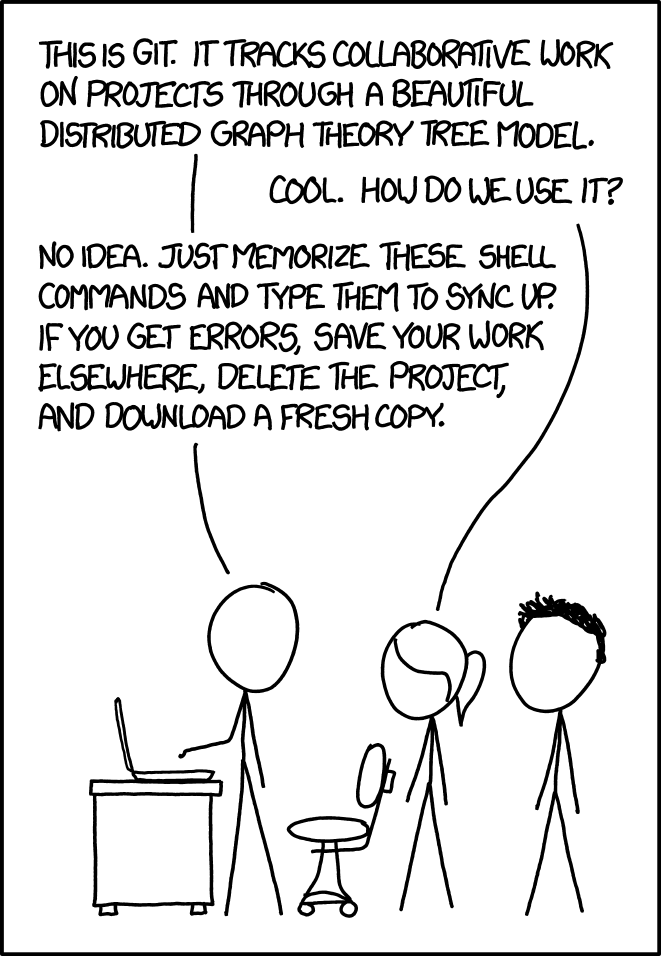
\includegraphics[width=0.5\textwidth]{figures/git_2x.png}
\end{frame}

\begin{frame}{What is a revision control system (RCS)}
\titleline
{\small
  Software needs to be \textcolor{blue}{maintained},
 \textcolor{blue}{debugged}, \textcolor{blue}{improved}...
while keeping track of the changes and being able to recover old revisions if needed.
\medskip

Those task can be done automatically using a \textcolor{red}{Revision Control System}.
\medskip

In addition, one may want to keep a copy of the code (and of all its changes) in a remote repository, for safety and for sharing with others.

\smallskip

Most common RCS: CVS, RCS, git, mercurial (Hg)....
}
\titleline
\end{frame}

\begin{frame}{Centralised vs Distributed RCS}
\begin{minipage}{0.45\textwidth}
\includegraphics[width=\textwidth]{figures/centralised}
\end{minipage}
\hfill
\begin{minipage}{0.45\textwidth}
\includegraphics[width=\textwidth]{figures/distributed}
\end{minipage}
\medskip

Centralised RCS compares with a distributed RCS as an \textcolor{blue}{hub} compares with a \textcolor{blue}{peer--to--peer} model.
\end{frame}
\begin{frame}{The concept of a distributed RCS}
\begin{itemize}
\item Each user has a \textcolor{red}{local copy of the repository}: you have full control of the history of the changes even if you are not connected to the web;
\item Most commands \alert{operate on the local copy} (minimize communications);
\item You may have \alert{multiple remote repositories}: good for distributed development.
\end{itemize}
\end{frame}


\begin{frame}{A Distributed RCS: git}
\titleline
{%
\small
\RaggedRight
Git is a distributed revision control system with an emphasis on speed.
It was initially designed and developed by Linus Torvalds for Linux kernel development. 
\smallskip

\alert{Every Git working directory is a full-fledged repository
with complete history and full revision tracking capabilities, not dependent on network access or a central server.}
}%
\titleline

In git (almost) every command operates just on the  \textcolor{red}{local}
repository. Indeed \textcolor{blue}{you do not even need a remote repository to use git!}.
\titleline
\end{frame}

\begin{frame}{A snapshot of this repo (using gitk)}
  \includegraphics[width=\textwidth]{figures/gitSnapshot}
\end{frame}

\begin{frame}{A snapshot of this repo (using gitk)}
  \includegraphics[width=\textwidth]{figures/gitk1}
\end{frame}
\begin{frame}{A snapshot of this repo (using gitk)}
  \includegraphics[width=\textwidth]{figures/gitk2}
\end{frame}
\begin{frame}{A snapshot of this repo (using gitk)}
  \includegraphics[width=\textwidth]{figures/gitk3}
\end{frame}

\begin{frame}{Free remote repos}
\begin{itemize}
    \item \href{https://github.com/}{Github}
    \item \href{https://gitlab.com/}{GitLab}
    \item \href{https://bitbucket.org/}{Bitbucket}
\end{itemize}
\end{frame}

\begin{frame}{Graphical Interfaces}
There are plenty of graphical interfaces for git. I sometimes use \href{https://git-cola.github.io/}{git-cola}, but you may find many others on the web.
A list may be found \href{https://git-scm.com/download/gui/linux}{here}.

\medskip

\centerline{
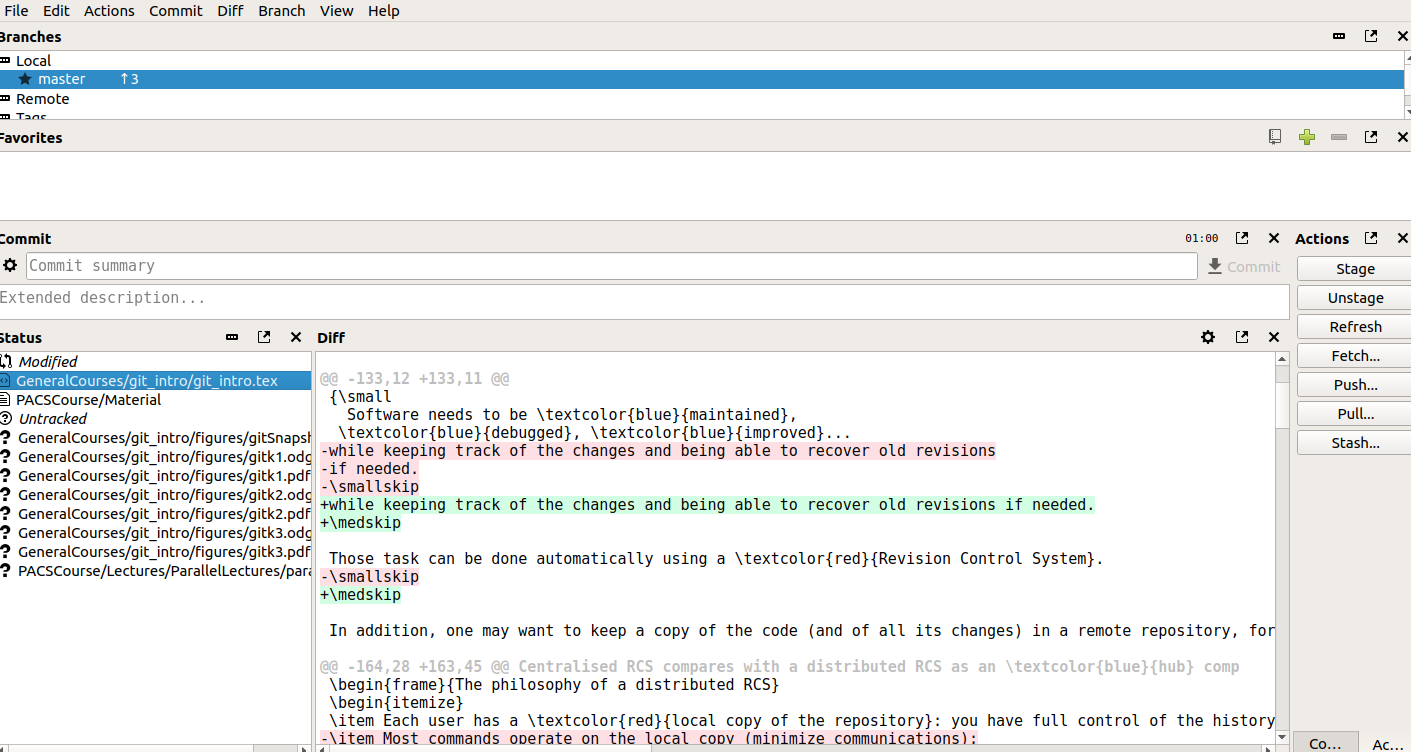
\includegraphics[width=0.9\textwidth]{figures/gitcola}
}

\end{frame}
% %%%%%%%%%%%%%%%%%%%%%%%%%%%%%%%%%%%%%%%%%%%%%%%%%
% \begin{frame}{A graphic approach}
% \begin{center}
% 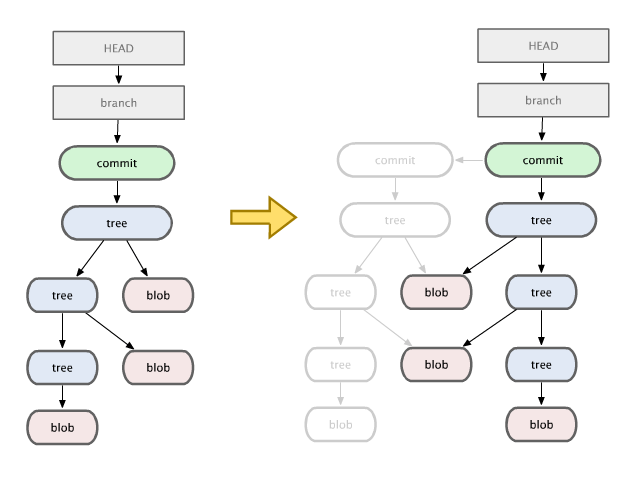
\includegraphics[width=.8\textwidth]{figures/git_trees}
% \end{center}
% \end{frame}
%%%%%%%%%%%%%%%%%%%%%%%%%%%%%%%%%%%%%%%%%%%%%%%%%
%\begin{frame}{Commands that communicate with a remote repository}
%Even if you do not yet know what they do, here there are the main %three commands used by git to operate on a remote repository:
%\medskip
%
%\begin{center}
%\alert{push, fetch, pull}
%\end{center}
%
%All other commands operate only on the local repository.
%\end{frame}

\begin{frame}{First thing to do}
If you have never used git on a computer you should first \alert{let git know who you are}  (so people can blame you for your wrong deeds or cherish you for your programming skill!)

\begin{shell}
\psone git config -{}-global user.name ``Micky Mouse''
\end{shell}
\begin{shell}
  \psone git config -{}-global user.email \nl
  ``micky.mouse@gmail.com''
\end{shell}

\texttt{git config} tells git to change some git configuration. 
\texttt{global} makes it to change parameters that applies to all yours git repo in that computer.  \titleline
\end{frame}

\begin{frame}{Other useful global setting}
\titleline
Git is highly configurable, for instance, if you want to set for git a different editor than the system default one
\begin{shell}
\psone git config -{}-global core.editor emacs
\end{shell}
This command will set the default editor for git to \texttt{emacs}.
\titleline
\end{frame}

\begin{frame}{Need help?}
\titleline

Git has an integrated help. If you need help for the command \texttt{command}
just do

\begin{shell}
\psone git help command 
\end{shell}

Git uses a lot of terms that may confuse you at the beginning (and not only at the beginning...). A useful command is 

\begin{shell}
\psone git help glossary
\end{shell}

You find more on the \href{http://git-scm.com/book}{Git Book (git-scm.com/book)}
\titleline
\end{frame}

\begin{frame}{More help?}
  \titleline
  Other useful commands:
\begin{shell}
\psone git help tutorial
\end{shell}
A tutorial
\begin{shell}
\psone git help tutorial-2
\end{shell}
The second part of the tutorial.
\titleline

Git is a very complete (and complex) revision system, \alert{don't be scared:} in fact you will normally need just a few commands.
\end{frame}


\begin{frame}{Create/clone a repo}
Create a brand new local repository. In the directory where you want to create it type:
\begin{shell}
\psone git init
\end{shell}
\smallskip

Often you want to clone of an existing remote repository (on \textcolor{blue}{GitHub} in this example).
\medskip

\textcolor{blue}{With \texttt{https} protocol} (simpler but more limited):
\begin{shell}
\psone git clone \nl https://github.com/pacs-course/pacs.git
\end{shell}
\textcolor{blue}{With \texttt{ssh} protocol} (you need a github account where you have provided your public ssh key):
\begin{shell}
  \var{username}@github.com:/pacs-course/pacs.git
\end{shell}
\end{frame}

%%%%%%%%%%%%%%%%%%%%%%%%%%%%%%%%%%%%%%%%%%%%%%%%% 
%\begin{frame}{Protocols for connection to remotes}
%\begin{center}
%\begin{tabular}{ccccc}
%PROTOCOL      & PORT & READ & WRITE & PUBLIC \\
%\hline \\
%\tshell{ssh}  & 22   & YES  & YES   & NO     \\
%\tshell{git}  & 9418 & YES  & YES   & YES/NO \\
%\tshell{http} & 80   & YES  & NO    & YES    \\
%\end{tabular}
%
%\vspace{1cm}
%not exclusive! You may even send repository changes via mail or using a USB stick! 
%\end{center}
%\end{frame}
%%%%%%%%%%%%%%%%%%%%%%%%%%%%%%%%%%%%%%%%%%%%%%%%%
\begin{frame}{Edit!}
Modify some files in the repo
\begin{shell}
\psone edit the sources \ldots \\
\end{shell}
show status of the repo
\begin{shell}
\psone git status \\
\tiny%
\# On branch \var{branch_name} \\
\# Changes to be committed: \\
\#   (use "git reset HEAD <file>..." to unstage) \\
\# \\
\#       modified:   file1.cpp \\
\# \\
\# Changed but not updated: \\
\#   (use "git add <file>..." to update what will be committed) \\
\#   (use "git checkout -{}- <file>..." to discard changes in working directory) \\
\# \\
\#       modified:   file2.cpp \\
\# \\
\# Untracked files: \\
\#   (use "git add <file>..." to include in what will be committed) \\
\# \\
\#       file3.cpp \\
\end{shell}
\end{frame}

\begin{frame}{The possible state of a file in the working directory}
\begin{itemize}
\item \alert{untracked} The file is \textcolor{blue}{not under git control}. Maybe it is just a temporary file. Or maybe you want to put it under control using \textcolor{blue}{\texttt{git add <file>}}.

\item \alert{modified} The file has been modified since the last \textcolor{blue}{commit} in the repository. May be you want to \texttt{add} it to the staging area with \textcolor{blue}{\texttt{git add <file>}}.

\item \alert{staged} (in the index, or staging area). Ready to be \textcolor{blue}{committed} into the repository with a \textcolor{blue}{\texttt{git commit}}.
\end{itemize}
\end{frame}
\begin{frame}{The git workflow}
  \centerline{\includegraphics[width=0.75\textwidth]{figures/gitareas}}
  
  \alert{\texttt{.git}} is the \alert{hidden directory} where \texttt{git} stores its internal database and configuration files. \alert{DON'T DELETE IT!!}\\[3mm]
  
  See also: \url{https://ndpsoftware.com/git-cheatsheet.html}
\end{frame}

%%%%%%%%%%%%%%%%%%%%%%%%%%%%%%%%%%%%%%%%%%%%%%%%%
\begin{frame}{Add and Commit}
stage files for a commit
\begin{shell}
\psone git add \var{edited_files}
\end{shell}
create a new commit in the repository
\begin{shell}
\psone git commit \\
\ldots \\
<a editor will come up,\\ write a description for the commit>
\end{shell}
or
\begin{shell}
\psone git commit -m "message"\\
\end{shell}
The last command writes the commit message directly.
\end{frame}

\begin{frame}{What to put in a commit message}
\titleline
\begin{shell}
A first line with a brief description (it is the one that is shown by some git commands)\\
\vspace{0.3cm}

Possibly followed by an empty line and a detailed description (possibly wrap lines to 72 characters)\\
\vspace{0.3cm}
 
Paragraphs are separated by empty lines.\\
\vspace{0.3cm}
 
- you may create lists using the - character
\end{shell}
\titleline
If you use the option \texttt{-m} \alert{you can only set the brief description} (often it is enough!).
\end{frame}

\begin{frame}{What is git?}
  \centering
  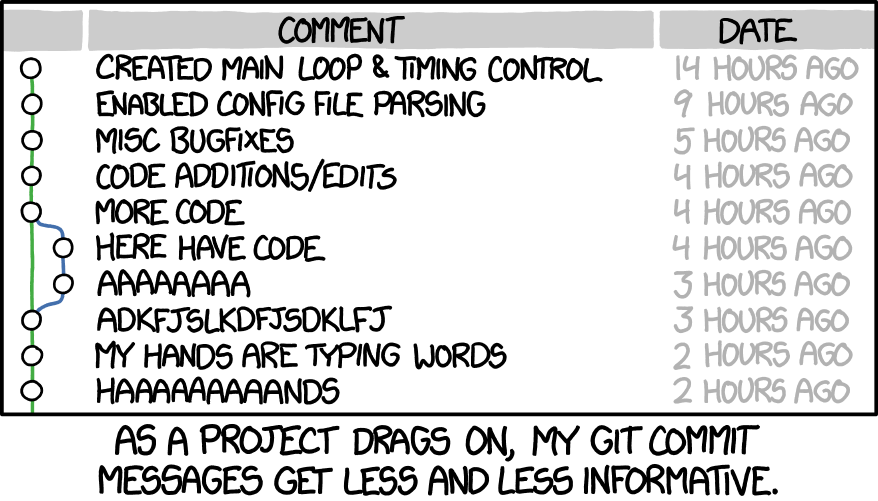
\includegraphics[width=0.95\textwidth]{figures/git_commit_2x.png}
\end{frame}

\begin{frame}{Add, Commit}
  \vspace*{-0.3cm}
\titleline
To recall, the basic operations are
\begin{itemize}
\item \alert{git add file(s)} Add a snapshot of the file(s) to the staging area ready for commit. On a \textcolor{blue}{new file}, it adds also the file to the git history.
\item \alert{git commit} Stores the staging area into the git \textcolor{blue}{local repository} creating a new \textcolor{blue}{commit}.
\end{itemize}
\titleline

\begin{shell}
\psone git commit -a 
\end{shell}
\textcolor{blue}{commits all modified files (but not the newly created, untracked, ones)}
\titleline
\end{frame}
%\begin{frame}{A graphical view}
%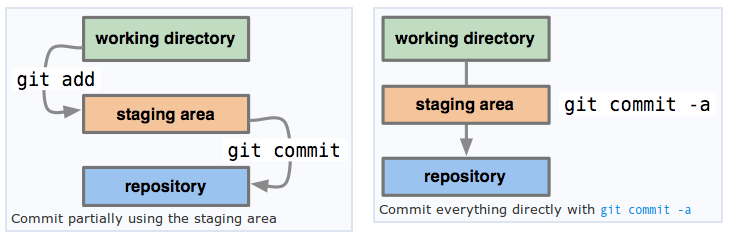
\includegraphics[width=\textwidth]{figures/commit}
%\end{frame}


\begin{frame}{Adding whole directories}
\titleline
If you have a directory with new (or modified) files doing

\begin{shell}
\psone git add DirectoryName
\end{shell} 
will \texttt{add} to the staging area all new (or modified) files in that directory.
\titleline

\alert{Note:} git operates on files: \textcolor{red}{trying to add an empty directory just does nothing!}
\end{frame}


\begin{frame}{What is a commit}
\titleline
A commit can be thought as a \alert{snapshot of your git working area at the moment of the commit.} It is identified by a unique \alert{hash key},  generated automatically.
\smallskip

\textcolor{red}{Any part of the hash key (as long as unique in the repo)} can be used to address a commit. A commit may also have symbolic names called \textcolor{blue}{tags}, created with \texttt{git tag <tagname>}.

\begin{shell}
\psone git show 
\end{shell}
shows the most recent commit (on the current branch).
\end{frame}

\begin{frame}{Some shorthand names for commits}
  \vspace*{-0.5cm}
\begin{center}
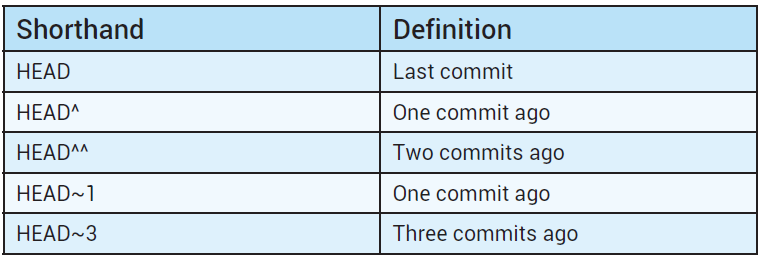
\includegraphics[width=0.75\textwidth]{figures/commitsShortHand}
\end{center}
{\small
These shorthands can be used in all git commands that refer to a commit. \textcolor{blue}{\texttt{HEAD} may be thought as a pointer to the last commit.}
\begin{shell}
\psone git log  HEAD\textasciitilde 3..HEAD\\
\psone git checkout HEAD\textasciitilde 2
\end{shell}
The first command prints a brief log describing the last 4 commits. The second positions your working area to two commits ago.
}
\end{frame}


\begin{frame}
  \frametitle{Checking-out a commit}
\titleline
  \begin{shell}
    \psone git checkout <treeish> 
  \end{shell}

  Where \texttt{treeish} can be:
  \begin{itemize}
  \item The \textcolor{blue}{hash key} of a commit, or a \texttt{tag} name;
  \item The name of a \textcolor{blue}{branch}: it will checkout the
    last commit (\texttt{HEAD}) of that branch;
  \item The \textcolor{blue}{shorthand} name of a commit.
  \end{itemize}
\titleline
\end{frame}

\begin{frame}{Important}
  \titleline
  If you checkout a commit that is not \texttt{HEAD} of a branch (we
  will deal with branches soon!) then you are put to a \alert{detached
    HEAD state}. You can modify files but not make
  commits! If you want to commit changes made while in detached \texttt{HEAD} state you have to create a branch:
  \small
  \begin{shell}
\psone git checkout HEAD\textasciitilde{}1

Note: checking out 'HEAD\textasciitilde{}1'.

You are in 'detached HEAD' state. You can look around, make experimental
changes and commit them, and you can discard any commits you make in this
state without impacting any branches by performing another checkout.

If you want to create a new branch to retain commits you create, you may
do so (now or later) by using -b with the checkout command again. Example:

  git checkout -b <new-branch-name>

HEAD is now at f041086 Added lecture on C++ evolution
  \end{shell}

\end{frame}
%%%%%%%%%%%%%%%%%%%%%%%%%%%%%%%%%%%%%%%%%%%%%%%% 
\begin{frame}{Fixing commits: amend reset and revert}
Sometimes you want to correct your \alert{last commit}, for instance to add some additional stuff, correcting the commit message ..., without creating a new commit
\begin{shell}
\psone <do your additional work/add/rm>\\
\psone git commit -{}-amend
\end{shell}
\smallskip

\alert{Never amend a commit that has been already pushed to a remote repo: use git revert}
\end{frame}

\begin{frame}{Eliminating modifications on files}
  \titleline
  The command \textcolor{blue}{\texttt{checkout}} can be used to bring a file to the version at a specified \texttt{commit}
\begin{shell}
\psone git checkout <commit> -{}- file(s)
\end{shell}
Brings file(s) at the state at \texttt{<commit>} (\texttt{<commit>} can be a branch or tag name).
\alert{Local modifications are lost}. If \texttt{<commit>} is missing, you can omit the \texttt{-{}-} and git considers the \texttt{HEAD} of the current branch. It means that you are discarding \alert{any modification} of the file since the last commit.
\titleline
\end{frame}

\begin{frame}{Undo staging}
\titleline
\texttt{git reset} sets yours HEAD to a specified commit. But it is a very versatile command
\titleline
\begin{shell}
\psone git reset <file>
\end{shell}

Removes the specified file (all if \texttt{<file>} is empty) from the staging area, \alert{leaving the working directory unchanged}.
\titleline

\textcolor{blue}{It is the opposite of \texttt{git add}.}

\end{frame}

\begin{frame}{Eliminating commits but not the changes}
  \titleline
\begin{shell}
\psone git reset <commit>
\end{shell}
Move back to \textcolor{blue}{<commit>}, \alert{leaving the working directory alone:} \textcolor{blue}{ all changes made since \texttt{<commit>} will be in the working directory, not staged}.
\titleline
\end{frame}

\begin{frame}{Hard Reset: bring history back!}
\begin{shell}
\psone git reset -{}-hard <commit>
\end{shell}
{\small Move the current branch tip backward to \texttt{<commit>} and reset both the staging area and the working directory to match. You are back at the situation at commit \texttt{<commit>}.
\alert{All modifications since \texttt{<commit>} are lost.}
}
\medskip 

\begin{shell}
\psone git reset -{}-hard
\end{shell}
{\small
Equivalent to \texttt{git reset -{}-hard HEAD}.  In addition to unstaging files, Git will \alert{overwrite all changes in the working directory.} \alert{All uncommitted changes are obliterated}, and you go back to the situation at your last commit.
}
\end{frame}

\begin{frame}{Reset and checkout}
    Note the difference between
\begin{shell}
  \psone git reset -{}-hard <commit>
\end{shell}
and
\begin{shell}
  \psone git checkout <commit>
\end{shell}

With \textcolor{blue}{\texttt{checkout}} the commits after \texttt{<commit>} (among
which \texttt{HEAD}) \alert{are still there}, that's why you are put
in a \emph{detached HEAD state}. \textcolor{blue}{\texttt{reset -{}-hard <commit>}} eliminates the commits following \texttt{<commit>} from the git history and sets \texttt{HEAD} to \texttt{<commit>}. \alert{All changes since\texttt{<commit>} are deleted.}
\titleline
\end{frame}

\begin{frame}{A warning}
\titleline
Reset may change the history. \alert{Do not use it to ``delete'' commits that have already been pushed to a remote repository shared with collaborators} (unless you want to loose friends).
\smallskip

\centering{\textcolor{blue}{\large Use \texttt{revert} in this case!.}}

\titleline

\end{frame}

\begin{frame}{Revert}
\texttt{git revert} reverts commits by \alert{playing them backwards}. So it does not ``delete'' them. It is history safe.
\begin{shell}
\psone git revert HEAD\textasciitilde{}3
\end{shell}
reverts the changes specified by the fourth last commit in HEAD and
          creates a new commit with the reverted changes.

\titleline
\begin{shell}
\psone git revert HEAD\textasciitilde{}3..HEAD
\end{shell}
reverts all changes introduced in the last four commits,
          creating a new commit with the reverted changes.
\titleline
\end{frame}
\begin{frame}{Ignoring files!}
  \titleline
  But often in your working directory you have files
  (temporary results, executables, libraries...) that you \alert{do
    not want to store in your repository}. You may just ignore them,
  but if you want to avoid making mistake (and stop \texttt{git
    status} indicating them as \textcolor{blue}{untracked}) you can
  create a \alert{\texttt{.gitignore}} file with the list of files to ignore (you can use wildcards)
  \titleline
  
  \alert{Remember to add and commit \texttt{.gitignore}, it must be in your repo!}
  \titleline

\end{frame}

\begin{frame}{Cleaning up!}
  \titleline
  All commands seen in the previous slides (like almost all git commands) operate on file under git control.
  Sometimes you want to get rid of \alert{untracked files} and have in your working area only
  the tracked one.
\begin{shell}
\psone git clean [-d] [-f] [-x]
\end{shell}

Option \texttt{-f} (force) is in fact \alert{compulsory}. With just that option the command cleans all untracked files not listed in \texttt{.gitignore} (the files in \texttt{.gitignore} are untracked but considered as \textcolor{blue}{known to git}.), with \texttt{-x} you get rid also of them. Directories emptied by the cleaning are kept unless you specify \texttt{-d}
\titleline

\textcolor{blue}{There are also other options: e.g. -i = interactive mode}

\end{frame}

\begin{frame}{Some advice}
\titleline
\begin{itemize}
\item \alert{Do atomic commits}: each commit should be related to a single ``logical change'' in your code: a bug fix, a new feature... \textcolor{blue}{Avoid monster commits with a lot of modified files.}
\item \alert{Write significant commit messages}. Messages like ``this is a commit'' are useless! A good message helps you to remember what you have done, and others understand your work. 
\item \textcolor{blue}{Git doesn't allow commits with empty messages.}
\end{itemize}
\titleline
\end{frame}





\begin{frame}{Branches}
\centerline{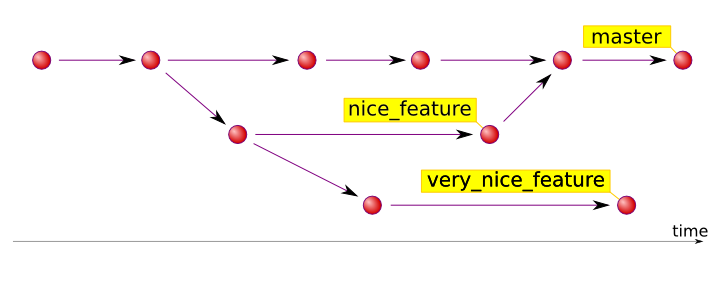
\includegraphics[width=0.7\textwidth]{figures/git-history}}

\titleline

\textcolor{red}{Branching is one of the most important feature of git.} 
When you create a repo you create also the \alert{\texttt{master}} branch. But often you want to create a branch to work on a specific topic (or just to experiment something) without affecting the master branch.
\end{frame}
%%%%%%%%%%%%%%%%%%%%%%%%%%%%%%%%%%%%%%%%%%%%%%%%%
\begin{frame}{Branching- create}
\titleline
create new branch
\begin{shell}
\psone git branch \var{shiny_new_branch} \\
\end{shell}
Go to that branch.
\begin{shell}
\psone git checkout \var{shiny_new_branch}
\end{shell}
Or create and position yourself in a new branch with a single command
\begin{shell}
\psone git checkout -b \var{shiny_new_branch}
\end{shell}
\titleline
\end{frame}

\begin{frame}{Get other branches}
list local branches
\begin{shell}
\psone git branch \\
~ b1\\
* b2\\
~ master
\end{shell}
list remote branches (i.e. branches fetched from remote, see fetching later on)
\begin{shell}
\psone git branch -r
\end{shell}
list all branches (local and remote)
\begin{shell}
\psone git branch -a
\end{shell}
\end{frame}
%%%%%%%%%%%%%%%%%%%%%%%%%%%%%%%%%%%%%%%%%%%%%%%%%
\begin{frame}{Branching  - delete}
delete a branch
\begin{shell}
\psone git checkout master \\
\psone git branch -d \var{branch_to_delete}
\end{shell}
will cause an error if the branch was not merged with master!

To delete it without merging with master
\begin{shell}
\psone git branch -D \var{branch_to_delete}
\end{shell}
To delete a remote branch (see later for remotes)
\begin{shell}
\psone git push origin :\var{branch_to_delete}
\end{shell}
\begin{center}
%\scriptsize%
%the syntax comes from the generic generic push command\\
%\tshell{git push \var{remotename} %\var{localbranch_name}:\var{remotebranch_name}}\\
%so we push an empty branch into the remote branch to be deleted
\end{center}
\end{frame}
%%%%%%%%%%%%%%%%%%%%%%%%%%%%%%%%%%%%%%%%%%%%%%%%%
\begin{frame}{Branching  - merge}
Often when you have finished working on a branch and you are happy of your work you want to merge the work on the \texttt{master} branch (or any other branch in fact).
\titleline
\smallskip

To merge a branch into master:
\begin{shell}
\psone git checkout master\\
\psone git merge \var{branch_name}\\
Updating e0f73f9..cd928c7\\
Fast-forward
\end{shell}
\pause
Everything was fine, but sometimes conflicts may arise!
\begin{shell}
CONFLICT (content): Merge conflict in file.cpp\\
Automatic merge failed; fix conflicts and then commit the result.
\end{shell}
\end{frame}

\begin{frame}{Why conflicts?}
  \titleline
  Git tries to do its best to merge the work you have done in the branch, but maybe in the meantime you or one of your collaborators have modified the same lines of the same file on \texttt{master} (or the branch to which you are merging).
\medskip

In that case you have a \alert{conflict}, git stops the merge and it is up to you to sort out the mess.
\smallskip

If you want to cancel the merge and go back to the situation just before:
\begin{shell}
\psone git merge -{}-abort
\end{shell}
\titleline

\end{frame}
%%%%%%%%%%%%%%%%%%%%%%%%%%%%%%%%%%%%%%%%%%%%%%%%% 
\begin{frame}[fragile]{Branching  - solve conflicts 1}
Manual solution. In the file with the conflict you have
\begin{shell}
\verb!<<<<<<<! HEAD\\
\ldots portion in the HEAD commit\\
=======\\
\ldots portion in the branch you are merging\\
\verb!>>>>>>>! branch_name\\
\end{shell}
Use your preferred editor and modify the file. Eventually you should eliminate the \verb!<<<<<! and \verb!>>>>! lines.
\titleline

There are several graphic tools to help you fixing conflicts, one is \href{http://meldmerge.org/}{\texttt{meld}}, that can activated using
\texttt{git mergetool}.
\end{frame}

% \begin{frame}[fragile]{Branching  - solve conflicts 2}
% Using a gui
% \titleline
% \begin{shell}
% \psone git mergetool -{}-tool=<tool>\\
% merge tool candidates: meld opendiff kdiff3 tkdiff xxdiff tortoisemerge gvimdiff diffuse ecmerge p4merge araxis emerge vimdiff
% \end{shell}
% You may use one of the tools indicated (you must have it installed). Some, like meld, are rather sophisticated and provide a nice graphical interface.
% \end{frame}
%%%%%%%%%%%%%%%%%%%%%%%%%%%%%%%%%%%%%%%%%%%%%%%%%
\begin{frame}[fragile]{Branching  - solve conflicts 2}
After you have fixed the conflicting files, you have to stage them
\begin{shell}
\psone git add file.cpp
\end{shell}
A commit is needed when all the conflicts are solved!
\begin{shell}
\psone git commit
\end{shell}
\end{frame}
%

\begin{frame}{A special branch: the stash}
Checkout with hanging modifications is forbidden!
\begin{shell}
\psone git checkout master\\
error: Your local changes to the following files would be overwritten by checkout: \ldots
\end{shell}
Instead of creating a branch we can stash modifications
\begin{shell}
\psone git stash save
\end{shell}
and bring them back
\begin{shell}
\psone git stash \{ pop | apply \}
\end{shell}
remember to clear the stash if you use apply, which does not delete the stash.
\begin{shell}
\psone git stash clear
\end{shell}
\end{frame}


%%%%%%%%%%%%%%%%%%%%%%%%%%%%%%%%%%%%%%%%%%%%%%%%%%%%%%%%%%%%
%%%%%%%%%%%%%%%%%%%%%%%%%%%%%%%%%%%%%%%%%%%%%%%%%%%%%%%%%%%%
\begin{frame}{Communicate with a remote repository}
\titleline

So far we have used commands that operate on the \textcolor{blue}{local repository}. To collaborate with others you need to communicate with a common \textcolor{blue}{remote} repository (on Github for instance).

To interact with a remote repository we have three main commands:
\alert{push}, \alert{fetch} and \alert{pull}.
\medskip
\titleline

We assume we have a single remote repository (called \texttt{origin}) and a single branch (\texttt{master}).

But you can have multiple remotes, and multiple remote branches, and give them the name you like!
\titleline
\end{frame}
\begin{frame}{Which remote}
  \titleline
  \alert{\texttt{origin}} is the name git gives by default
  to the remote repository when you \textcolor{blue}{clone}
  your git repo from a remote site
    \medskip
 
    You may change it.
  \titleline
\end{frame}


\begin{frame}{Which remote}
To see the remote repo you are currently using
\begin{shell}
\psone git remote -v 
\end{shell}
with the flag \texttt{-v} you have more verbose info. 
\smallskip

To add a remote
\begin{shell}
\psone git remote add \var{remote-name} url
\end{shell}
To delete a remote
\begin{shell}
\psone git remote remove remote-name
\end{shell}
To change the name
\begin{shell}
\psone git remote rename old-name new-name
\end{shell}
\end{frame}

\begin{frame}{Pushing a commit to the remote}
\begin{shell}
git push \var{remote-name} \var{branch}
\end{shell}
Pushes all the commits for branch \texttt{branch} (the current branch by default) onto the remote \texttt{remote-name}. If you have more than one remote, you have to indicate the name.
\titleline
\medskip

Beware: if one of your collaborators has already pushed some new commits to the remote, you have first to \textcolor{blue}{pull} them (or create a separate branch and push the branch).
\end{frame}




\begin{frame}{Fetch from the remote}
\titleline
\begin{shell}
\psone git fetch \var{remote-name}
\end{shell}
Fetches all the commits for the current branch in the remote repository
and store them \alert{locally} in \texttt{remotes/<remotename>/<branch>}
\titleline

You can then examine them (read only!) by doing
\begin{shell}
\psone git checkout remotes/origin/new-branch
\end{shell}

You can finally merge the commits into your master
\begin{shell}
\psone git checkout master\\
\psone git merge remotes/origin/new_branch
\end{shell}
\titleline
\end{frame}
\begin{frame}{Pull from the remote}
\begin{shell}
\psone git pull \var{remote-name} \var{branch}
\end{shell}

It is equivalent to \textcolor{blue}{\texttt{git fetch} followed by
\texttt{git merge}}. If you omit the branch and remote name you will pull all branches in the repository corresponding to your local branches.
\medskip

\alert{It is probably the most used command when you want to retrieve commits from a remote repository.} But if you want to examine the changes first, use \texttt{fetch} instead.
\end{frame}

\begin{frame}{add, commit, push pull...}
\centerline{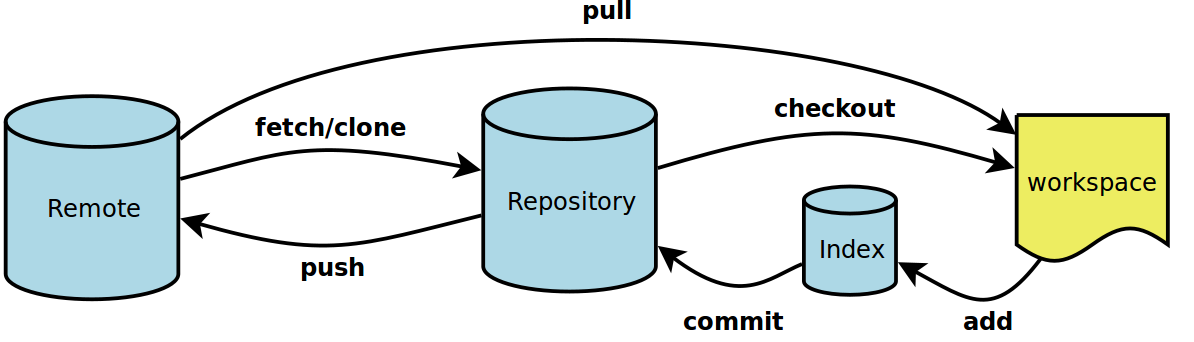
\includegraphics[width=\textwidth]{figures/pullandfetch}}
\end{frame}



%%%%%%%%%%%%%%%%%%%%%%%%%%%%%%%%%%%%%%%%%%%%%%%%%
\begin{frame}{Collaboration - remote}
Share a new branch with a remote called \texttt{repo_name}
\begin{shell}
\psone git push \var{repo_name} \var{branch_name}\\
\psone git pull \var{repo_name} \var{branch_name}
\end{shell}
Access a new branch in the repo after having fetched it
\begin{shell}
\psone git checkout -{}-track -b \var{branch_local_name} \nl \var{repo_name}/\var{branch_name}
\end{shell}

If you have just one repo it is sufficient to do
\begin{shell}
\psone git checkout -{}-track \var{branch_name}
\end{shell}
\vspace*{-0.4cm}
\titleline
{\small 
A \alert{tracking branch} is a branch that is linked to the corresponding branch in a remote repository. Indeed you may have \alert{local branches} just for local modifications.
}
\end{frame}

\begin{frame}{Remote branches}
  when you fetch or pull a branch from the remote git creates special branches with the name
  \begin{shell}
    remotes/<remotename>/<branchname>
  \end{shell}
  You can see them with
  \begin{shell}
    git branch -r
  \end{shell}
  and examine them with
  \begin{shell}
    git checkout remotes/<remotename>/<branchname>
  \end{shell}
  and merge them with a local branch.
  \titleline

  {\small\color{red}
    Beware, they are a local copy of the branches stored in the remote
    repo at the time of the last \texttt{fetch} or \texttt{pull}. }
\end{frame}

\begin{frame}{Get info}
  \titleline
\begin{shell}
\psone git log
\end{shell}
Shows commit logs.
\begin{shell}
\psone git shortlog
\end{shell}
Summarizes log output, showing commit description from each contributor 
\begin{shell}
\psone git show <object>
\end{shell}
Show some properties of the \texttt{object} (blob, commit...)
\titleline

\alert{Use a graphical interface like \texttt{gitk} or \texttt{git-cola}...}
\end{frame}

\begin{frame}{Other useful commands}
To show the differences with the last commit (you may specify a different commit and/or some specific files)
\begin{shell}
\psone git diff \var{branch} \var{files}
\end{shell}

To remove file(s) under git control from the working directory and stage it for removal in the next commit
\begin{shell}
\psone git rm file(s)
\end{shell}

To change the name of a file under git control (stages the change for the next commit)
\begin{shell}
\psone git mv oldname newname
\end{shell}
\end{frame}

\begin{frame}
  \Huge
  MORE ADVANCED ISSUES
\end{frame}
%%%%%%%%%%%%%%%%%%%%%%%%%%%%%%%%%%%%%%%%%%%%%%%%%% 

\begin{frame}{Merging and rebasing}
There are in fact two ways in git to integrate work from one branch into another: merge and rebase.

Rebase allow to keep a linear history, at the price of loosing the details of you reached a certain
configuration of your repository.
\end{frame}

%%%%%%%%%%%%%%%%%%%%%%%%%%%%%%%%%%%%%%%%%%%%%%%%%%
\begin{frame}{Merging and rebasing}
\begin{center}
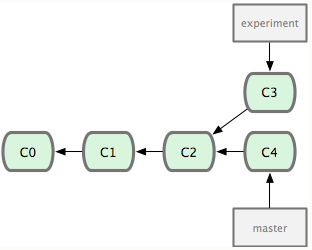
\includegraphics[width=0.6\textwidth]{figures/tomerge}
\end{center}
\end{frame}
\begin{frame}{I) Merge}
\begin{shell}
\psone git checkout master\\
\psone git merge experiment
\end{shell}
\begin{center}
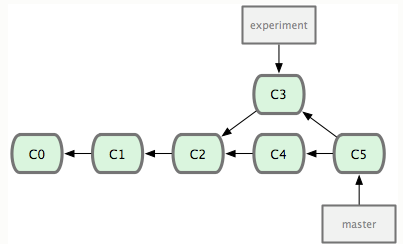
\includegraphics[width=0.7\textwidth]{figures/merged}
\end{center}
\end{frame}
\begin{frame}{II) Rebase}
\begin{shell}
\psone git checkout experiment\\
\psone git rebase master
\end{shell}
\begin{center}
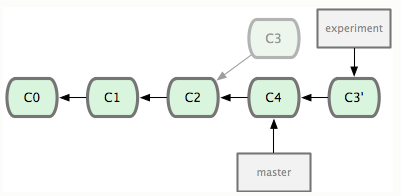
\includegraphics[width=0.8\textwidth]{figures/rebase1}
\end{center}
\end{frame}
\begin{frame}{II) And then  merge to realign master with experiment}
\begin{shell}
\psone git checkout master\\
\psone git merge experiment
\end{shell}
\begin{center}
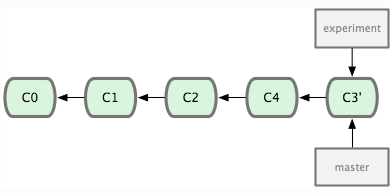
\includegraphics[width=0.8\textwidth]{figures/rebase2}\\
\end{center}
\end{frame}
%\begin{frame}{Rebase (alternative form)}
%\begin{shell}
%\psone git rebase master experiment\\
%\end{shell}
%\begin{center}
%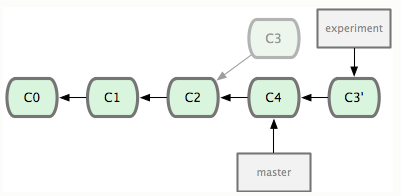
\includegraphics[width=0.8\textwidth]{figures/rebase1}\\
%\end{center}
%\end{frame}

\begin{frame}{The differences between merging and rebasing}
Merge does a three way merge. The history after the merge reflects what has happened. 
You create a commit with \alert{2 parents}.
\medskip

Rebase ``replays'' commits on the base on top of another branch. It will produce a \alert{linear history}, easier to read.
\medskip

Rebasing is also more general: you can select the commits to rebase (advanced topic not covered here).
\end{frame}

\begin{frame}{When merging? When rebasing?}
Rebase is useful if one wants to keep a linear history. It could be the method of choice to merge on a \alert{only local} branch work done in another branch.
\medskip
\titleline

\textcolor{blue}{Rebase however rewrites history, changing commits.} So 
\alert{you should never rebase on shared branches, where several developers are working (unless you like being hated).}
\end{frame}

%%%%%%%%%%%%%%%%%%%%%%%%%%%%%%%%%%%%%%%%%%%%%%%%% 
\begin{frame}{Some advanced features: submodules}
{\small
  A git repository may contain another git repository (and this 
  can be done recursively!). It is useful if you want to keep in your repository another, independent, project, so that you can use it and  update it if some useful changes happen upstream.
  
Example: you want to add to your repo a local copy of \texttt{https://github.com/PatWie/CppNumericalSolvers.git}.
\smallskip

Go to the directory where I want to store the submodule
\begin{shell}
\psone cd myrepo/numerical solvers
\end{shell}
\begin{shell}
\psone git submodule add https://github.com/PatWie/CppNumericalSolvers.git
\end{shell}
}

{\small
Now in \texttt{myrepo/dir/CppNumericalSolvers} you have a copy of the remote repo.
}
\end{frame}
%%%%%%%%%%%%%%%%%%%%%%%%%%%%%%%%%%%%%%%%%%%%%%%%% 
\begin{frame}{Operating on submodules}
You can update a submodule so that it is kept up-to-date with upstream
(\texttt{--recursive} is needed only if you have submodule of submodules)
\begin{shell}
\psone cd myrepo
\psone git submodule update --recursive
\end{shell}
Get info about submodules
\begin{shell}
\psone git submodule status
\psone git submodule summary
\end{shell}
\end{frame}
%%%%%%%%%%%%%%%%%%%%%%%%%%%%%%%%%%%%%%%%%%%%%%%%% 
\begin{frame}{Operating on submodules}
Remember that a submodule is a \alert{git repo!}
\begin{shell}
\psone cd myrepo/dir/CppNumericalSolvers
\psone git status
\end{shell}
I get the status of the git repository associated to \texttt{CppNumericalSolvers},
not of the hosting repository!

What if I clone \texttt{myrepo} somewhere else and I want to fetch also the submodules?
\begin{shell}
\psone git clone <myrepo> newrepo
\psone cd newrepo
\psone git submodule init
\psone git submodule update --recursive
\end{shell}
\end{frame}
%%%%%%%%%%%%%%%%%%%%%%%%%%%%%%%%%%%%%%%%%%%%%%%%
\begin{frame}
  \Huge
  \begin{center}
    Questions and Answers
  \end{center}
\end{frame}

%%%%%%%%%%%%%%%%%%%%%%%%%%%%%%%%%%%%%%%%%%%%%%%%% 
\begin{frame}{Common issues - I}
\boxltr{Q} edited on master branch by mistake, I wanted to do in new\_branch instead!

\boxltr{A} a simple checkout will do it
\begin{shell}
\psone git checkout -b new_branch
\end{shell}
\boxltr{Q} already committed to master branch

\boxltr{A} create a new branch and delete the commit on master
\begin{shell}
\psone git branch new_branch\\
\psone git reset -{}-hard HEAD\textasciitilde1\\
\psone git checkout new_branch\\
\end{shell}
\end{frame}

%%%%%%%%%%%%%%%%%%%%%%%%%%%%%%%%%%%%%%%%%%%%%%%%% 
\begin{frame}{Common issues - II}
\boxltr{Q} I want to discard my edit and get the latest version of the file!

\boxltr{A} Simple
\begin{shell}
\psone git checkout -{}- file
\end{shell}
\boxltr{Q} I want to get the file from another branch or another commit!

\boxltr{A} It's the same command as before:
\begin{shell}
\psone git checkout <branch|commit> -{}- file
\end{shell}
\end{frame}

%%%%%%%%%%%%%%%%%%%%%%%%%%%%%%%%%%%%%%%%%%%%%%%%%
\begin{frame}{Common issues - III}
\boxltr{Q} Get a commit from another branch

\boxltr{A} cherry-pick it to the correct one
\begin{shell}
\psone git checkout correct_branch\\
\psone git cherry-pick commit_hash
\end{shell}
\boxltr{Q} cannot get the branch of the local remote

\boxltr{A} Try with a fetch
\begin{shell}
\psone git fetch remote_name\\
\psone git remote show remote_name
\end{shell}
\end{frame}
%%%%%%%%%%%%%%%%%%%%%%%%%%%%%%%%%%%%%%%%%%%%%%%%%
\begin{frame}{Common issues - IV}
\boxltr{Q} the merge has gone bananas!

\boxltr{A} give up the merge and try again
\begin{shell}
\psone git merge \var{branch_to_be_merged}\\
\psone \#\$!\&\#\%\$\@\&\^\@ \\
\psone git reset -{}-hard \var{original_branch}
\end{shell}
or, more simply
\begin{shell}
git merge -{}-abort
\end{shell}

\boxltr{Q} i want a file from that branch!

\boxltr{A} get it with
\begin{shell}
\psone git checkout \var{branch} \var{files}\\
\end{shell}
\end{frame}
%%%%%%%%%%%%%%%%%%%%%%%%%%%%%%%%%%%%%%%%%%%%%%%%%
\begin{frame}{Common issues - V}
\boxltr{Q} git push refuses to work

\begin{shell}
\tiny
remote: error: refusing to update checked out branch: refs/heads/\var{branch_name}\\
remote: error: By default, updating the current branch in a non-bare repository\\
remote: error: is denied, because it will make the index and work tree inconsistent\\
remote: error: with what you pushed, and will require 'git reset -{}-hard' to match\\
remote: error: the work tree to HEAD.\\
remote: error:\\
remote: error: You can set 'receive.denyCurrentBranch' configuration variable to\\
remote: error: 'ignore' or 'warn' in the remote repository to allow pushing into\\
remote: error: its current branch; however, this is not recommended unless you\\
remote: error: arranged to update its work tree to match what you pushed in some\\
remote: error: other way.\\
remote: error:\\
remote: error: To squelch this message and still keep the default behaviour, set\\
remote: error: 'receive.denyCurrentBranch' configuration variable to 'refuse'.\\
To \var{repo}\\
 ! [remote rejected] \var{branch_name} -> \var{branch_name} (branch is currently checked out)\\
\end{shell}

\boxltr{A} use a bare repo
\begin{shell}
\psone git clone -{}-bare \var{repo} \var{repo}.git\\
\end{shell}
\begin{center}
\tiny\url{http://stackoverflow.com/questions/2199897/git-convert-normal-to-bare-repository}
\end{center}
\end{frame}
%%%%%%%%%%%%%%%%%%%%%%%%%%%%%%%%%%%%%%%%%%%%%%%%%
\begin{frame}[fragile]{Tips \& tricks - I}
\begin{itemize}%[<+->]
\item \tshell{gitk} is your friend
\item do small, atomic commits
\item read git output
\item branch in the prompt: add to \texttt{.bashrc}
\begin{shell}
\tiny
function GitBranch \{\\
~~\verb!_branch="$(git branch 2>/dev/null | sed -e "/^\s/d"!\\
~~\verb!-e "s/^\*\s//")"!\\
~~\verb!test -n "$_branch" && echo -e "@$_branch"!\\
\}\\
PS1=\textquotesingle\verb!\u@\h:\w$(GitBranch)> !\textquotesingle
\end{shell}
\vspace*{0.25cm}
\item watch out for non history-safe commands after pushing!
{\footnotesize(\tshell{cherry-pick},\texttt{reset},\tshell{rebase},\ldots)}
\item everything else (and more\ldots) on git
\begin{center}
\url{http://book.git-scm.com/index.html}
\end{center}
\end{itemize}
\end{frame}
%%%%%%%%%%%%%%%%%%%%%%%%%%%%%%%%%%%%%%%%%%%%%%%%%
\begin{frame}{Tips \& tricks - II}
\begin{itemize}%[<+->]
\item bash autocompletion
\begin{center}
\footnotesize
\url{http://git.kernel.org/?p=git/git.git;a=blob_plain;f=contrib/completion/git-completion.bash;hb=HEAD}
\end{center}
\item colored output
\begin{shell}
\psone git config -{}-global color.ui true
\end{shell}
\vspace*{0.25cm}
\item no empty push
\begin{shell}
\psone git config -{}-global push.default nothing
\end{shell}
\vspace*{0.25cm}
\item creating archives with the content of a commit
\begin{shell}
\psone git archive \var{commit_or_branch} | gzip > \nl \var{archive_name}.tgz
\end{shell}
\end{itemize}
\end{frame}
%%%%%%%%%%%%%%%%%%%%%%%%%%%%%%%%%%%%%%%%%%%%%%%%%
\end{document}

%%% Local Variables:
%%% mode: latex
%%% TeX-master: t
%%% End:
